\documentclass[11pt, a4paper]{article}
\usepackage{pdfpages}
\usepackage{parallel}
\usepackage[T2A]{fontenc}
\usepackage{ucs}
\usepackage[utf8x]{inputenc}
\usepackage[polish,english,russian]{babel}
\usepackage{hyperref}
\usepackage{rotating}
\usepackage[inner=2cm,top=1.8cm,outer=2cm,bottom=2.3cm,nohead]{geometry}
\usepackage{listings}
\usepackage{graphicx}
\usepackage{wrapfig}
\usepackage{longtable}
\usepackage{indentfirst}
\usepackage{array}
\usepackage{tikzsymbols}
\usepackage{soul}
\usepackage[ruled,vlined]{algorithm2e}
%\counterwithout{figure}{section} 

\usepackage{url}
\makeatletter
\g@addto@macro{\UrlBreaks}{\UrlOrds}
\makeatother

\newcolumntype{P}[1]{>{\raggedright\arraybackslash}p{#1}}
\frenchspacing
\usepackage{fixltx2e} %text sub- and superscripts
\usepackage{icomma} % коскі ў матэматычным рэжыме
\PreloadUnicodePage{4}

\newcommand{\longpage}{\enlargethispage{\baselineskip}}
\newcommand{\shortpage}{\enlargethispage{-\baselineskip}}

\def\switchlang#1{\expandafter\csname switchlang#1\endcsname}
\def\switchlangbe{
\let\saverefname=\refname%
\def\refname{Літаратура}%
\def\figurename{Іл.}%
}
\def\switchlangen{
\let\saverefname=\refname%
\def\refname{References}%
\def\figurename{Fig.}%
}
\def\switchlangru{
\let\saverefname=\refname%
\let\savefigurename=\figurename%
\def\refname{Литература}%
\def\figurename{Рис.}%
}

\hyphenation{admi-ni-stra-tive}
\hyphenation{ex-pe-ri-ence}
\hyphenation{fle-xi-bi-li-ty}
\hyphenation{Py-thon}
\hyphenation{ma-the-ma-ti-cal}
\hyphenation{re-ported}
\hyphenation{imp-le-menta-tions}
\hyphenation{pro-vides}
\hyphenation{en-gi-neering}
\hyphenation{com-pa-ti-bi-li-ty}
\hyphenation{im-pos-sible}
\hyphenation{desk-top}
\hyphenation{elec-tro-nic}
\hyphenation{com-pa-ny}
\hyphenation{de-ve-lop-ment}
\hyphenation{de-ve-loping}
\hyphenation{de-ve-lop}
\hyphenation{da-ta-ba-se}
\hyphenation{plat-forms}
\hyphenation{or-ga-ni-za-tion}
\hyphenation{pro-gramming}
\hyphenation{in-stru-ments}
\hyphenation{Li-nux}
\hyphenation{sour-ce}
\hyphenation{en-vi-ron-ment}
\hyphenation{Te-le-pathy}
\hyphenation{Li-nux-ov-ka}
\hyphenation{Open-BSD}
\hyphenation{Free-BSD}
\hyphenation{men-ti-on-ed}
\hyphenation{app-li-ca-tion}

\def\progref!#1!{\texttt{#1}}
\renewcommand{\arraystretch}{2} %Іначай формулы ў матрыцы зліпаюцца з лініямі
\usepackage{array}

\def\interview #1 (#2), #3, #4, #5\par{

\section[#1, #3, #4]{#1 -- #3, #4}
\def\qname{LVEE}
\def\aname{#1}
\def\q ##1\par{{\noindent \bf \qname: ##1 }\par}
\def\a{{\noindent \bf \aname: } \def\qname{L}\def\aname{#2}}
}

\def\interview* #1 (#2), #3, #4, #5\par{

\section*{#1\\{\small\rm #3, #4. #5}}
\ifx\ParallelWhichBox\undefined%
    \addcontentsline{toc}{section}{#1, #3, #4}%
\else%
\ifnum\ParallelWhichBox=0%
    \addcontentsline{toc}{section}{#1, #3, #4}%
\fi\fi%

\def\qname{LVEE}
\def\aname{#1}
\def\q ##1\par{{\noindent \bf \qname: ##1 }\par}
\def\a{{\noindent \bf \aname: } \def\qname{L}\def\aname{#2}}
}

\newcommand{\interviewfooter}[1]{
\vskip 1em
\noindent \textit{#1}
}


\begin{document}

\title{1993 "--- Colani Trackball}
\date{}
\maketitle

По всей видимости, Colani Trackball был первым среди так называемых <<дизайнерских>> манипуляторов, в разработке которых официально принимали участие звезды технического дизайна. Имя и форму данному конкретному устройству подарил Луиджи Колани (Luigi Colani) \cite{wiki}. Наибольшую известность Колани получил в области автоиндустрии, отметившись четырьмя десятками концепт-каров; не менее активно он проектировал мебель, предметы домашнего обихода, бытовую технику. Плодотворное сотрудничество Луиджи Колани с немецкой компанией Vobis Microcomputer, владельцем торговой марки Highscreen, привело к выпуску на основе его дизайна нескольких персональных компьютеров, джойстиков, мышей и трекболов.

\begin{figure}[h]
    \centering
    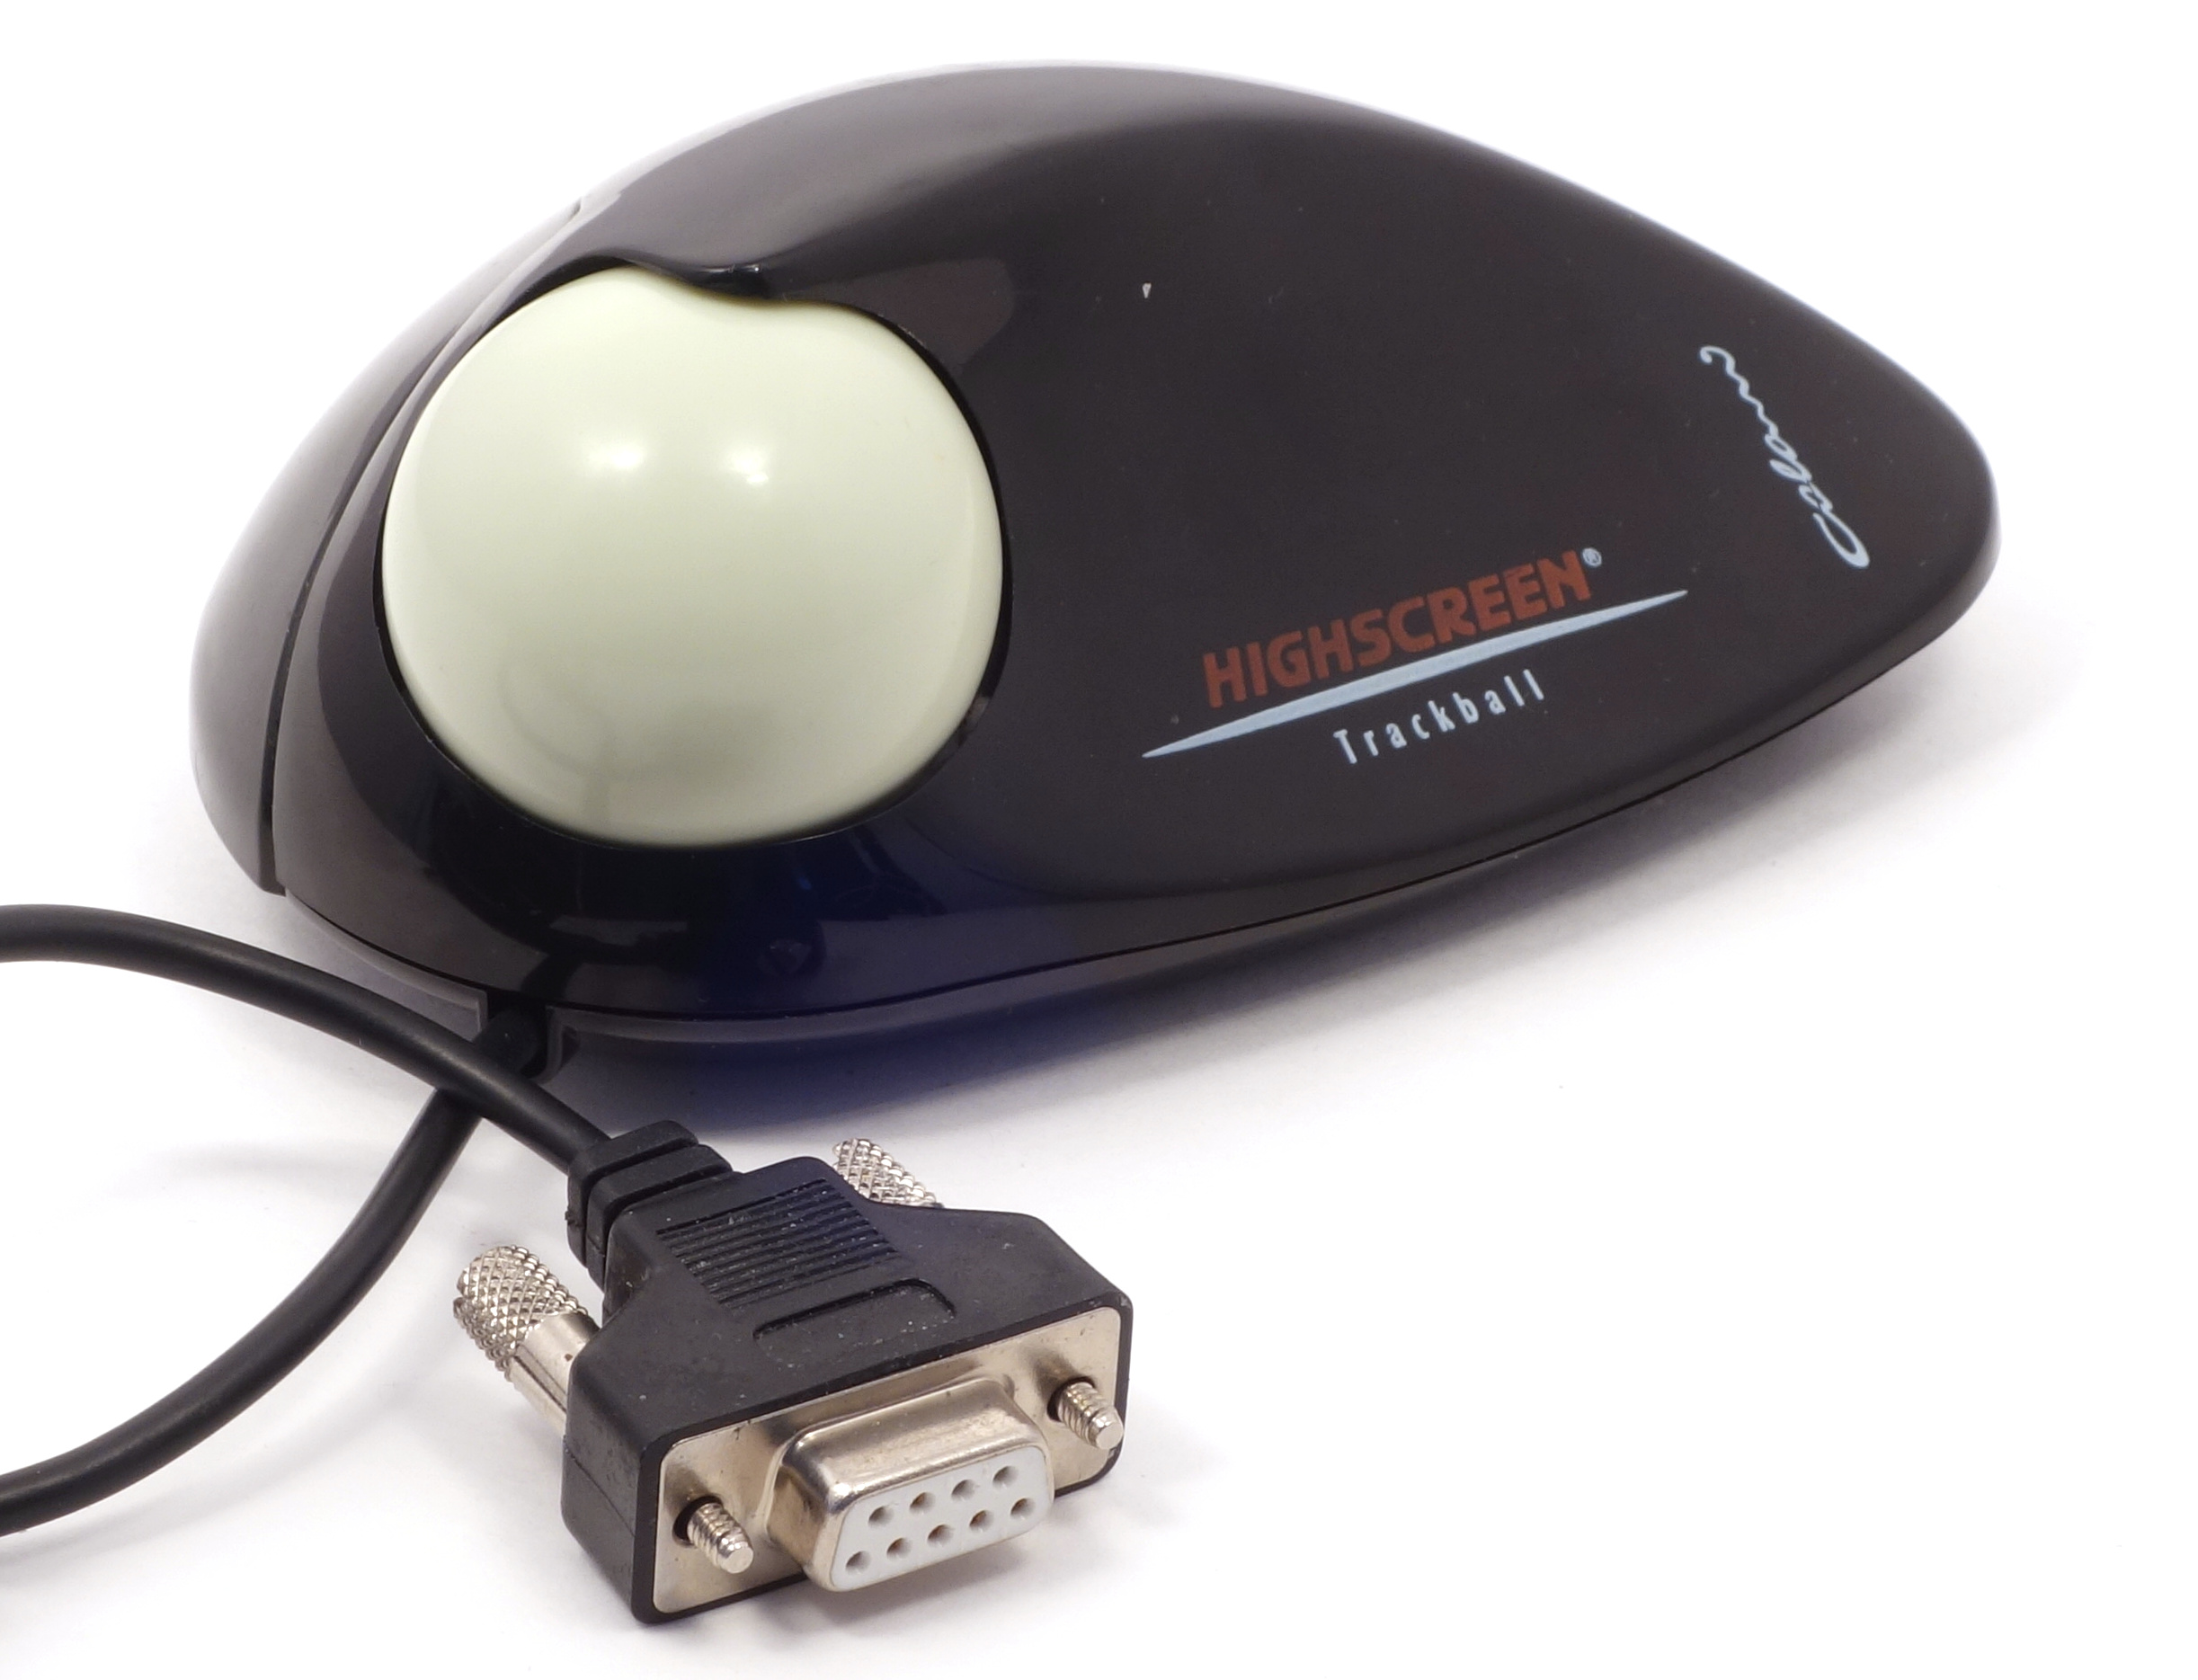
\includegraphics[scale=0.46]{1993_colani_trackball/pic_b_60.jpg}
    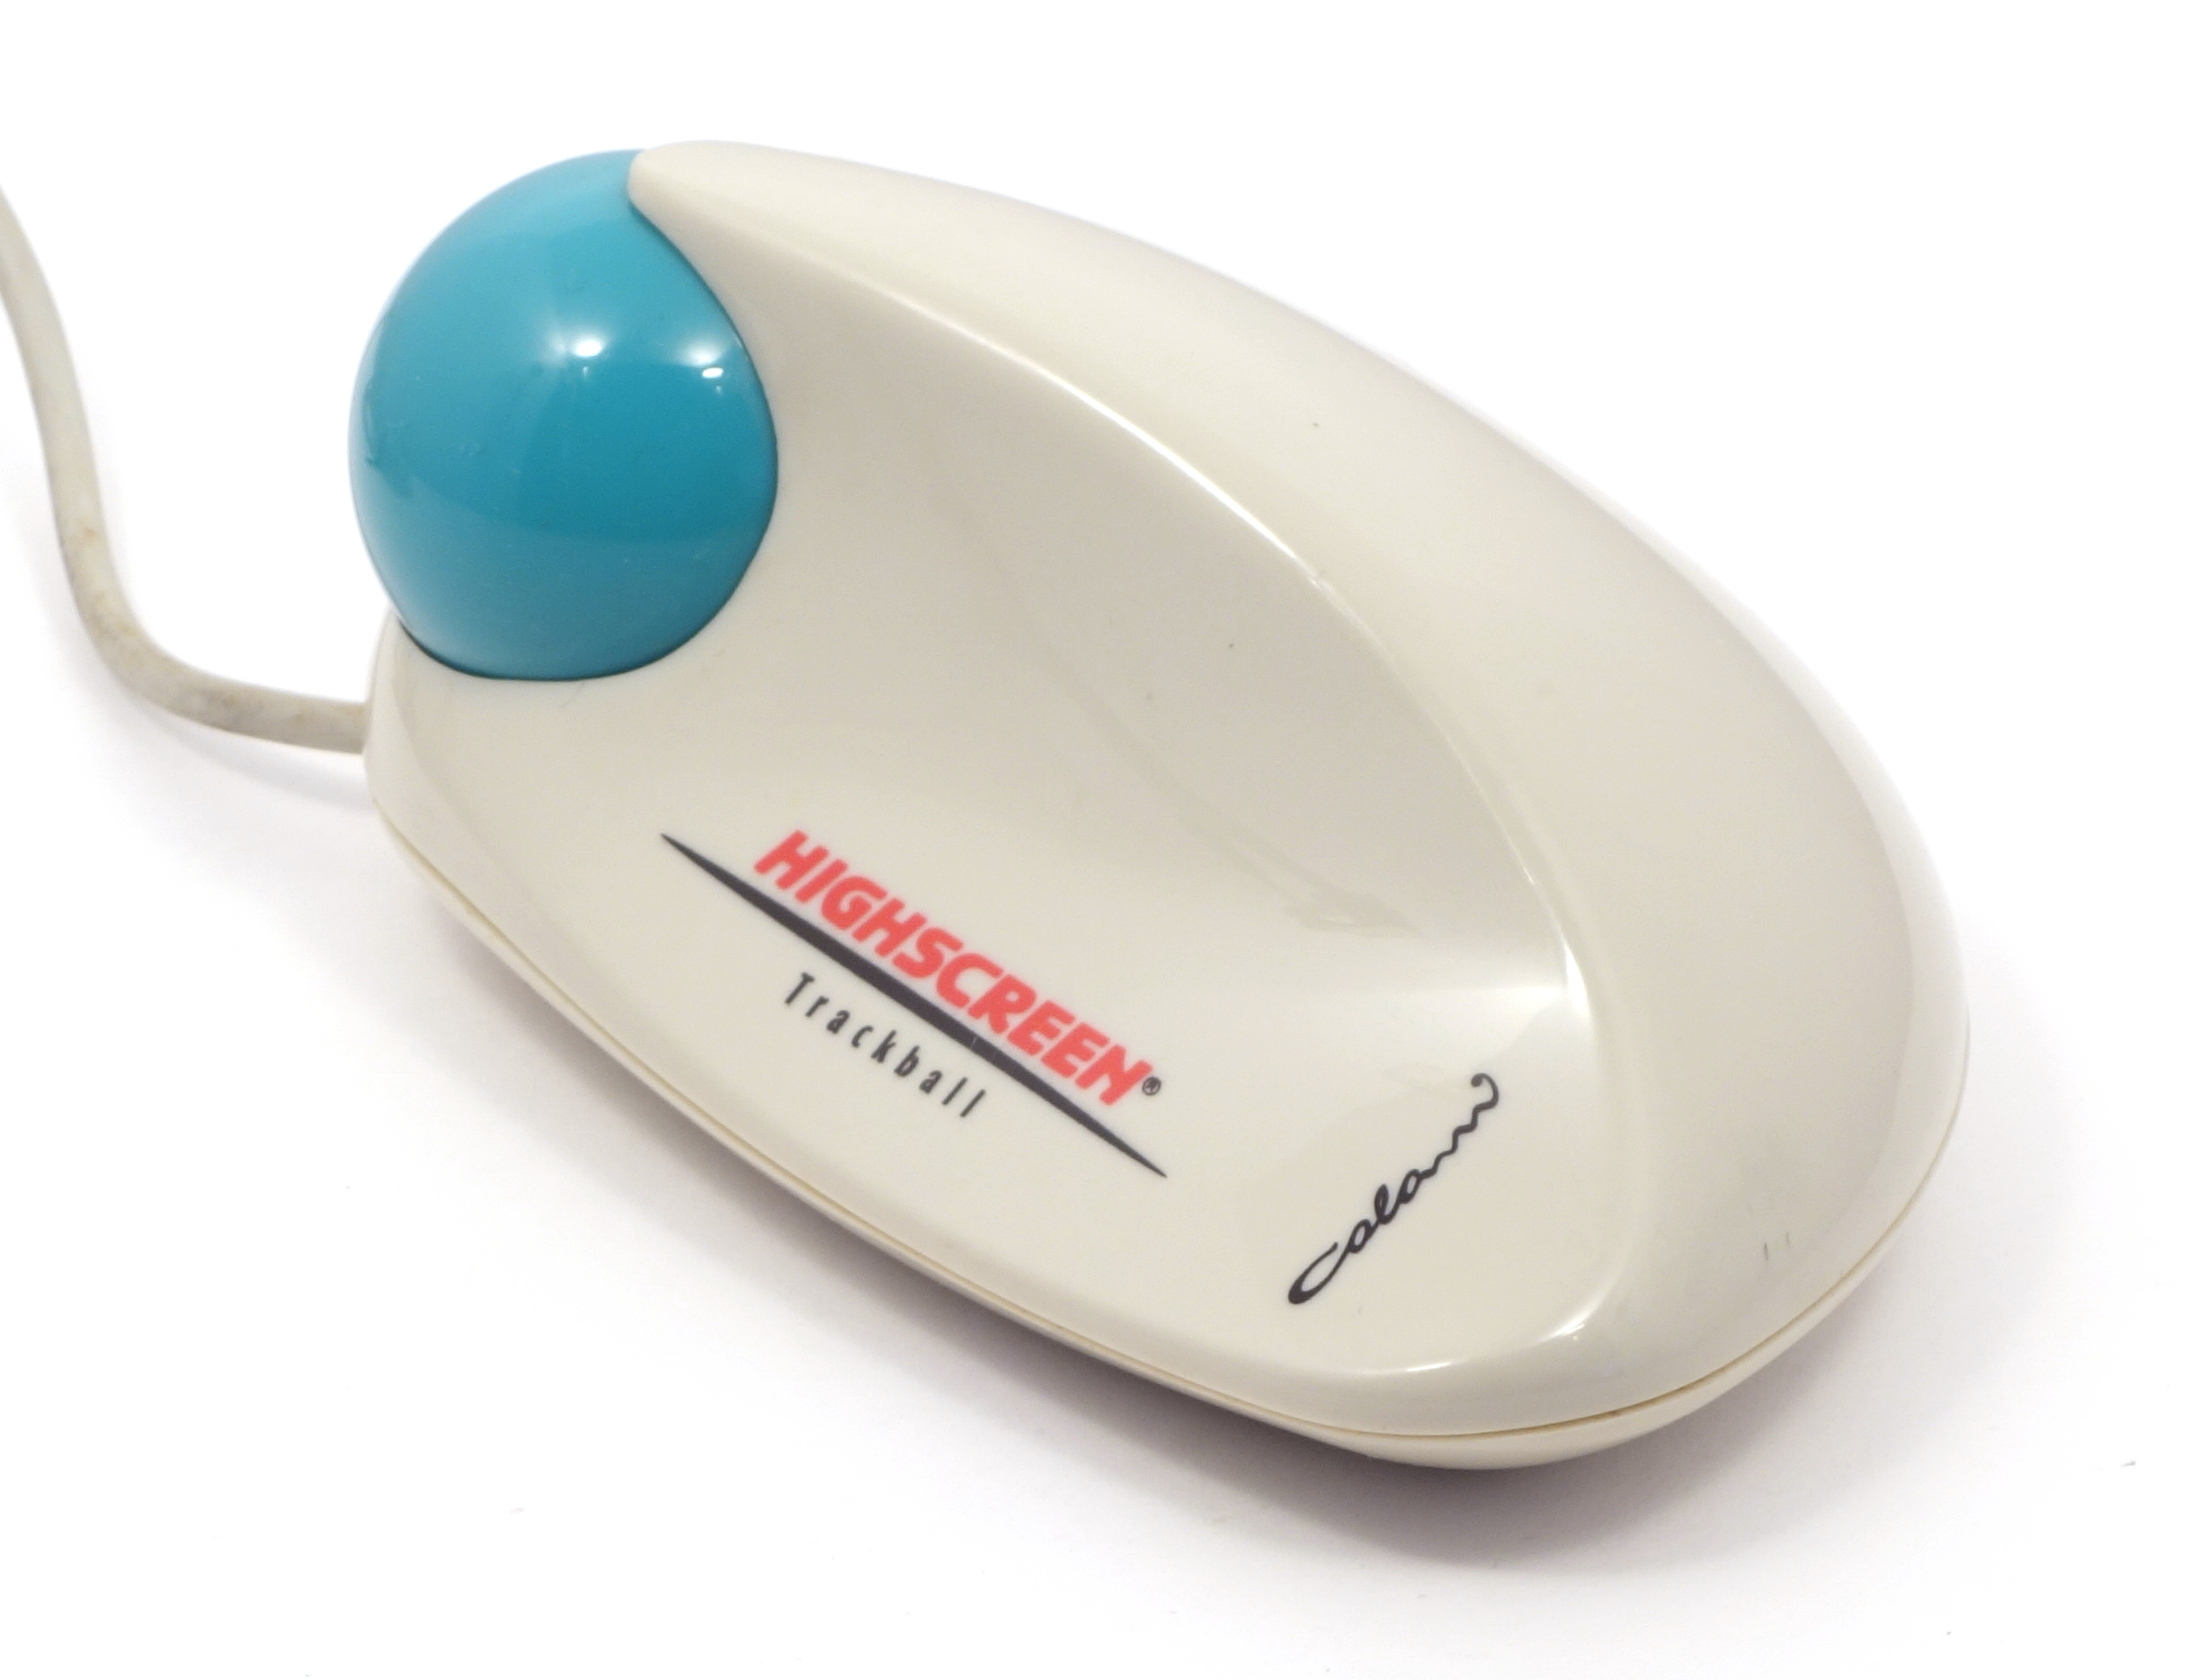
\includegraphics[scale=0.46]{1993_colani_trackball/pic_w_60.jpg}
    \caption{Colani Trackball}
    \label{fig:ColaniPic}
\end{figure}

HIGHSCREEN Colani Trackball, внешний вид которого показан на рис. \ref{fig:ColaniPic} "--- представитель этой линейки. Данная модель трекбола (вместе с мышью Colani Mouse того же производителя, имевшей сходный дизайн) выиграла престижную премию <<IF Design Award>> проектной организации «iF International Forum Design GmbH» в 1993 году \cite{award}. Трекбол выпускался в двух модификациях, отличавшихся цветом.

\begin{figure}[h]
    \centering
    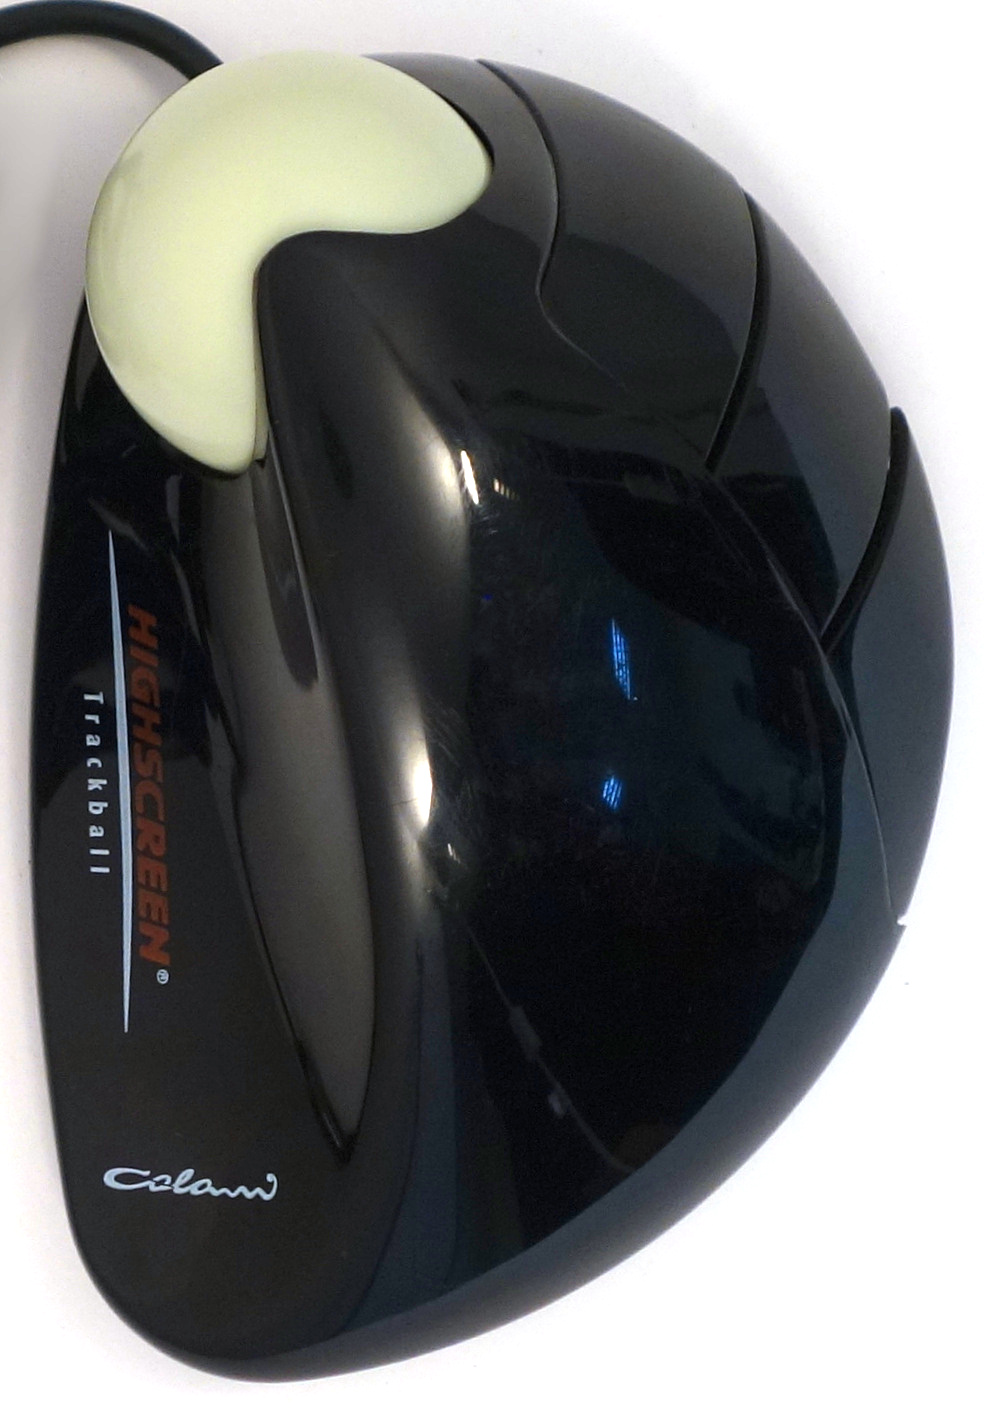
\includegraphics[scale=0.5]{1993_colani_trackball/top_b_30.jpg}
    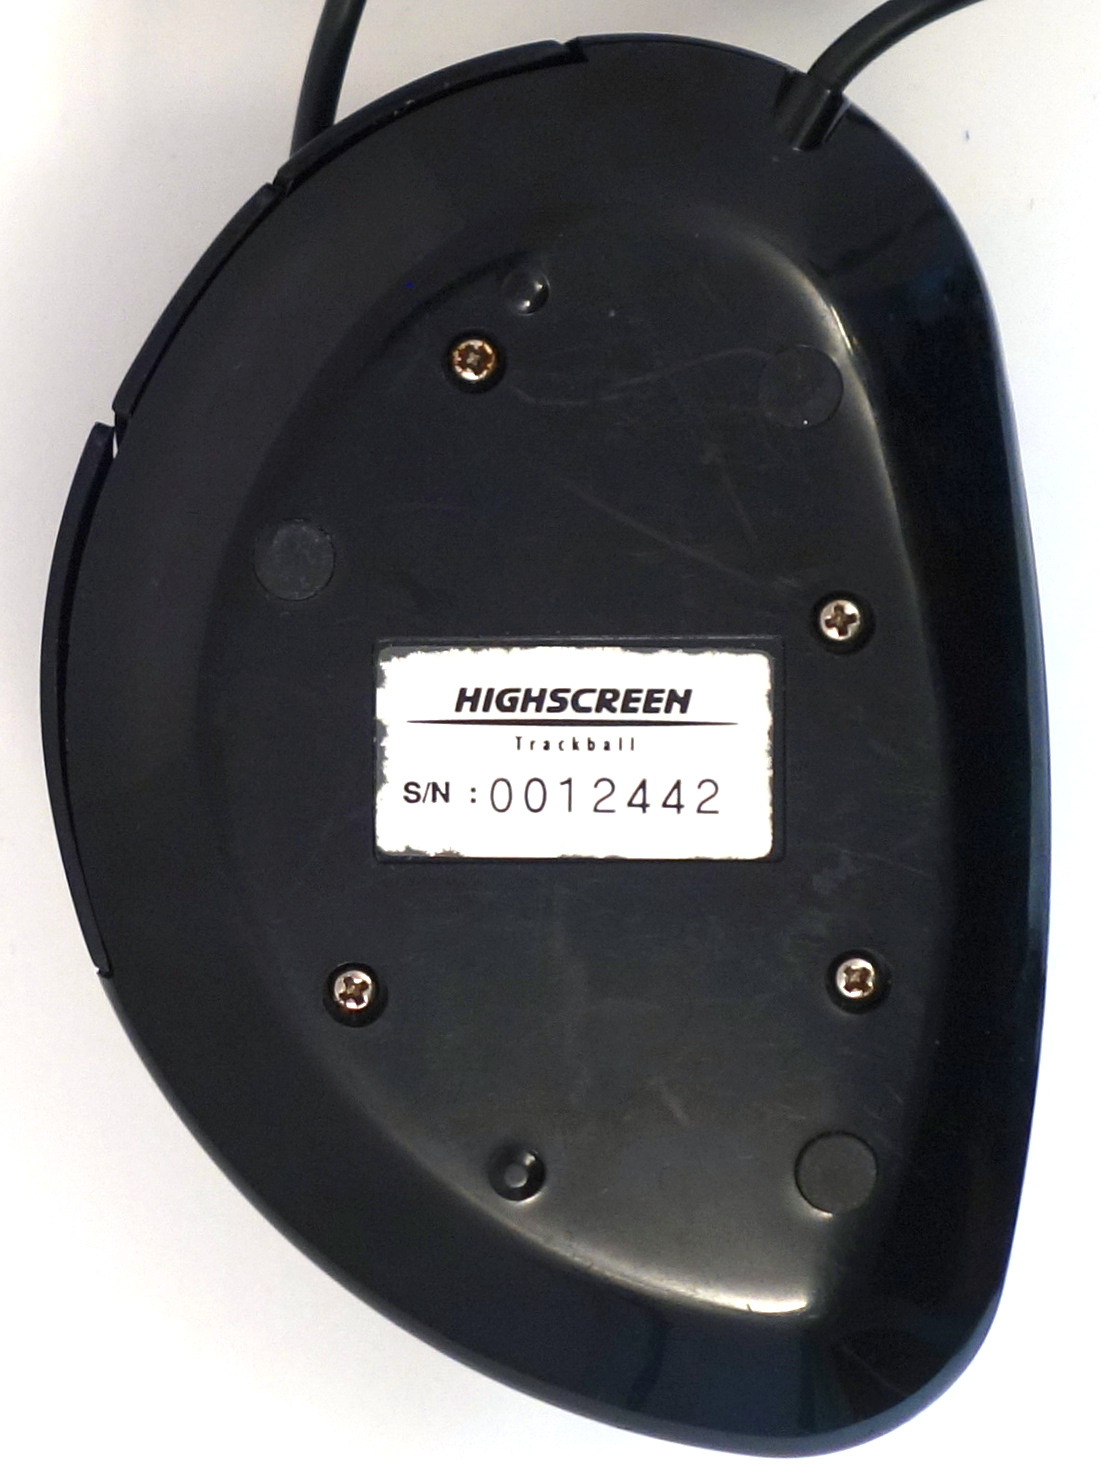
\includegraphics[scale=0.5]{1993_colani_trackball/bottom_b_30.jpg}
    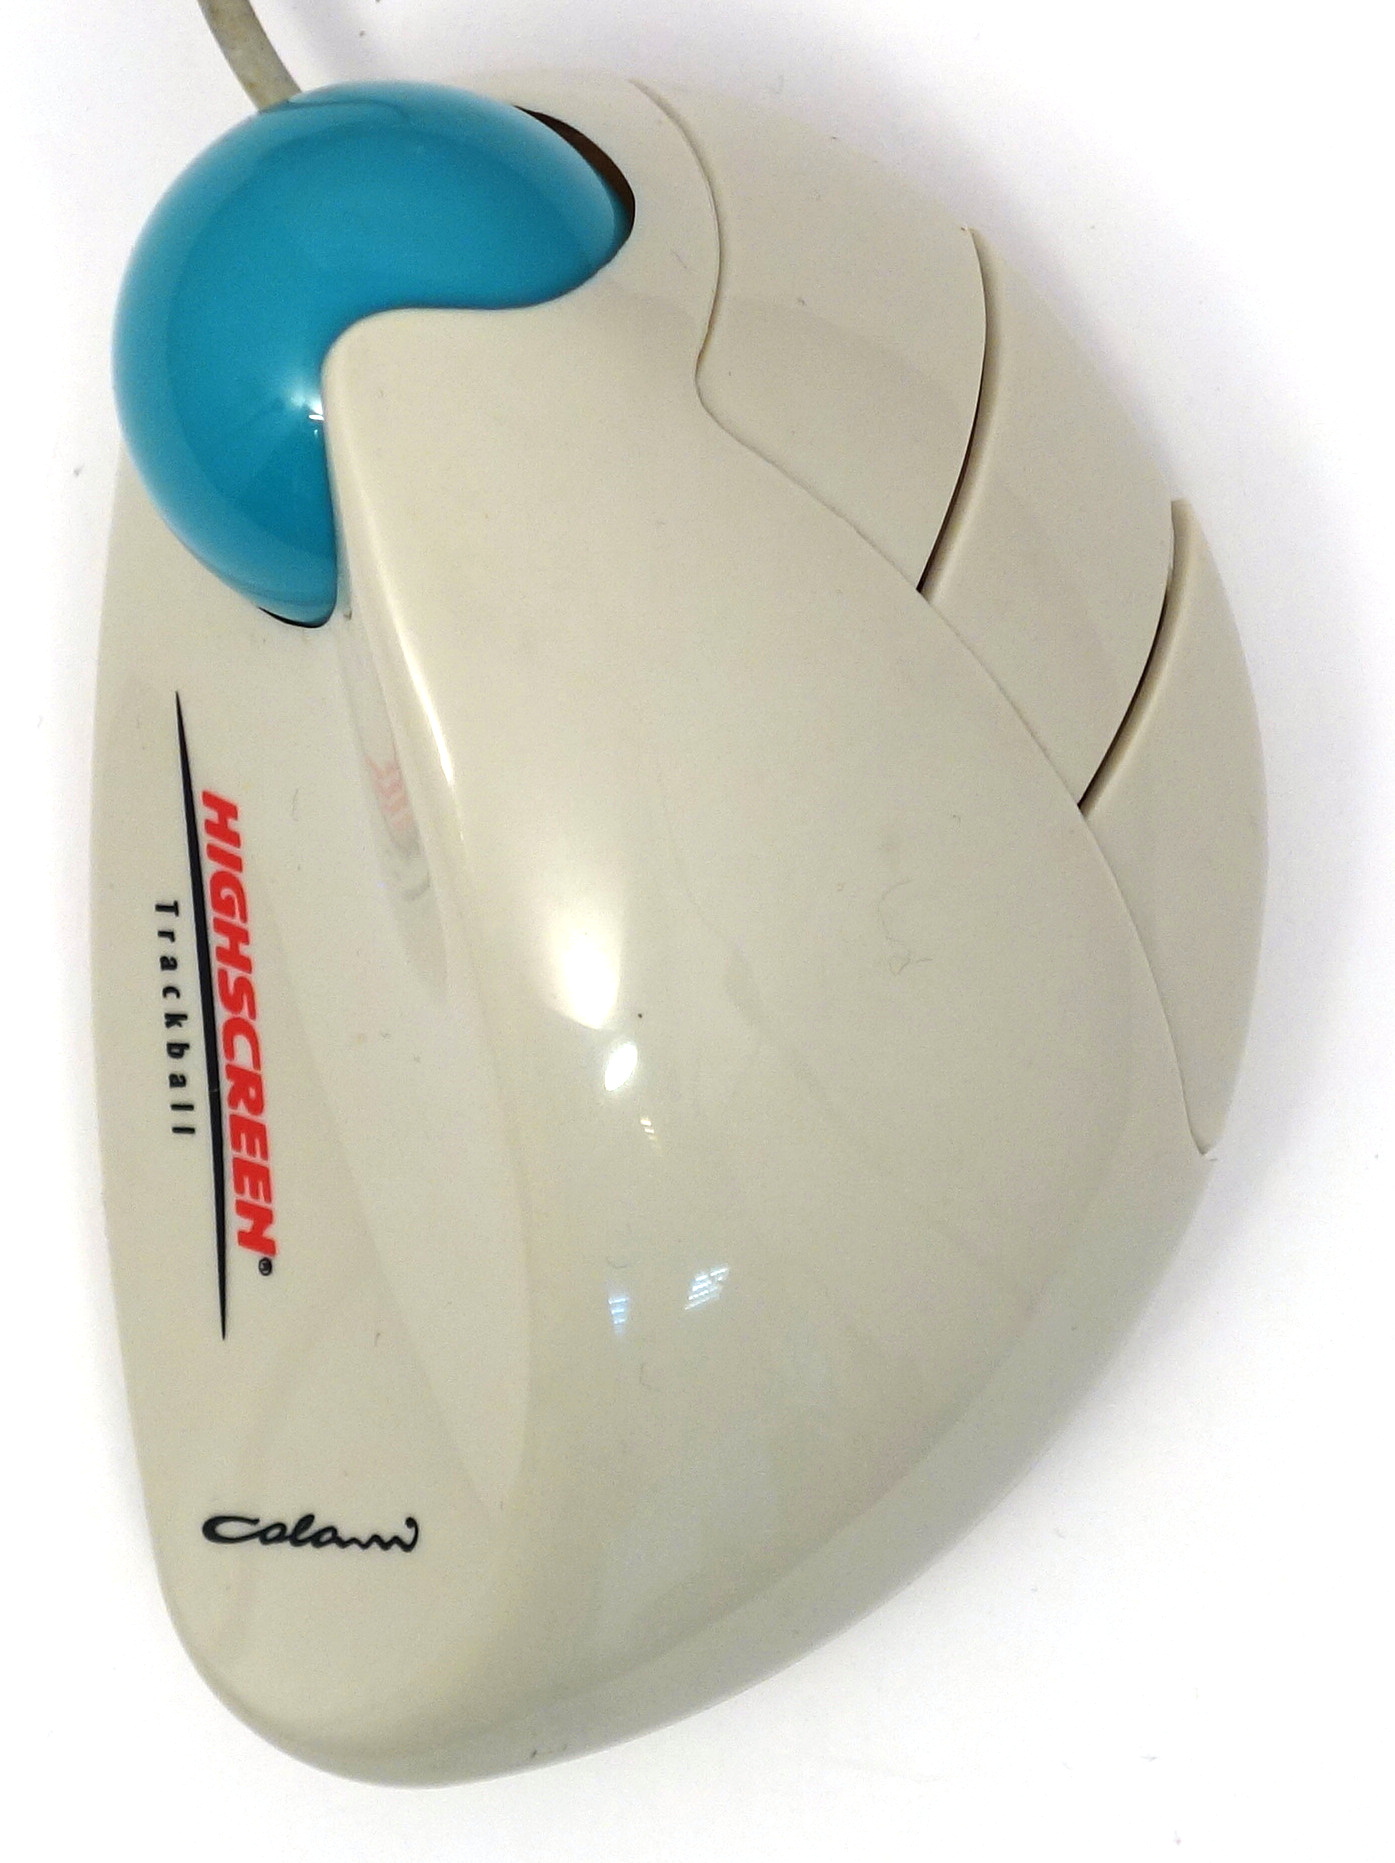
\includegraphics[scale=0.4]{1993_colani_trackball/top_w_30.jpg}
    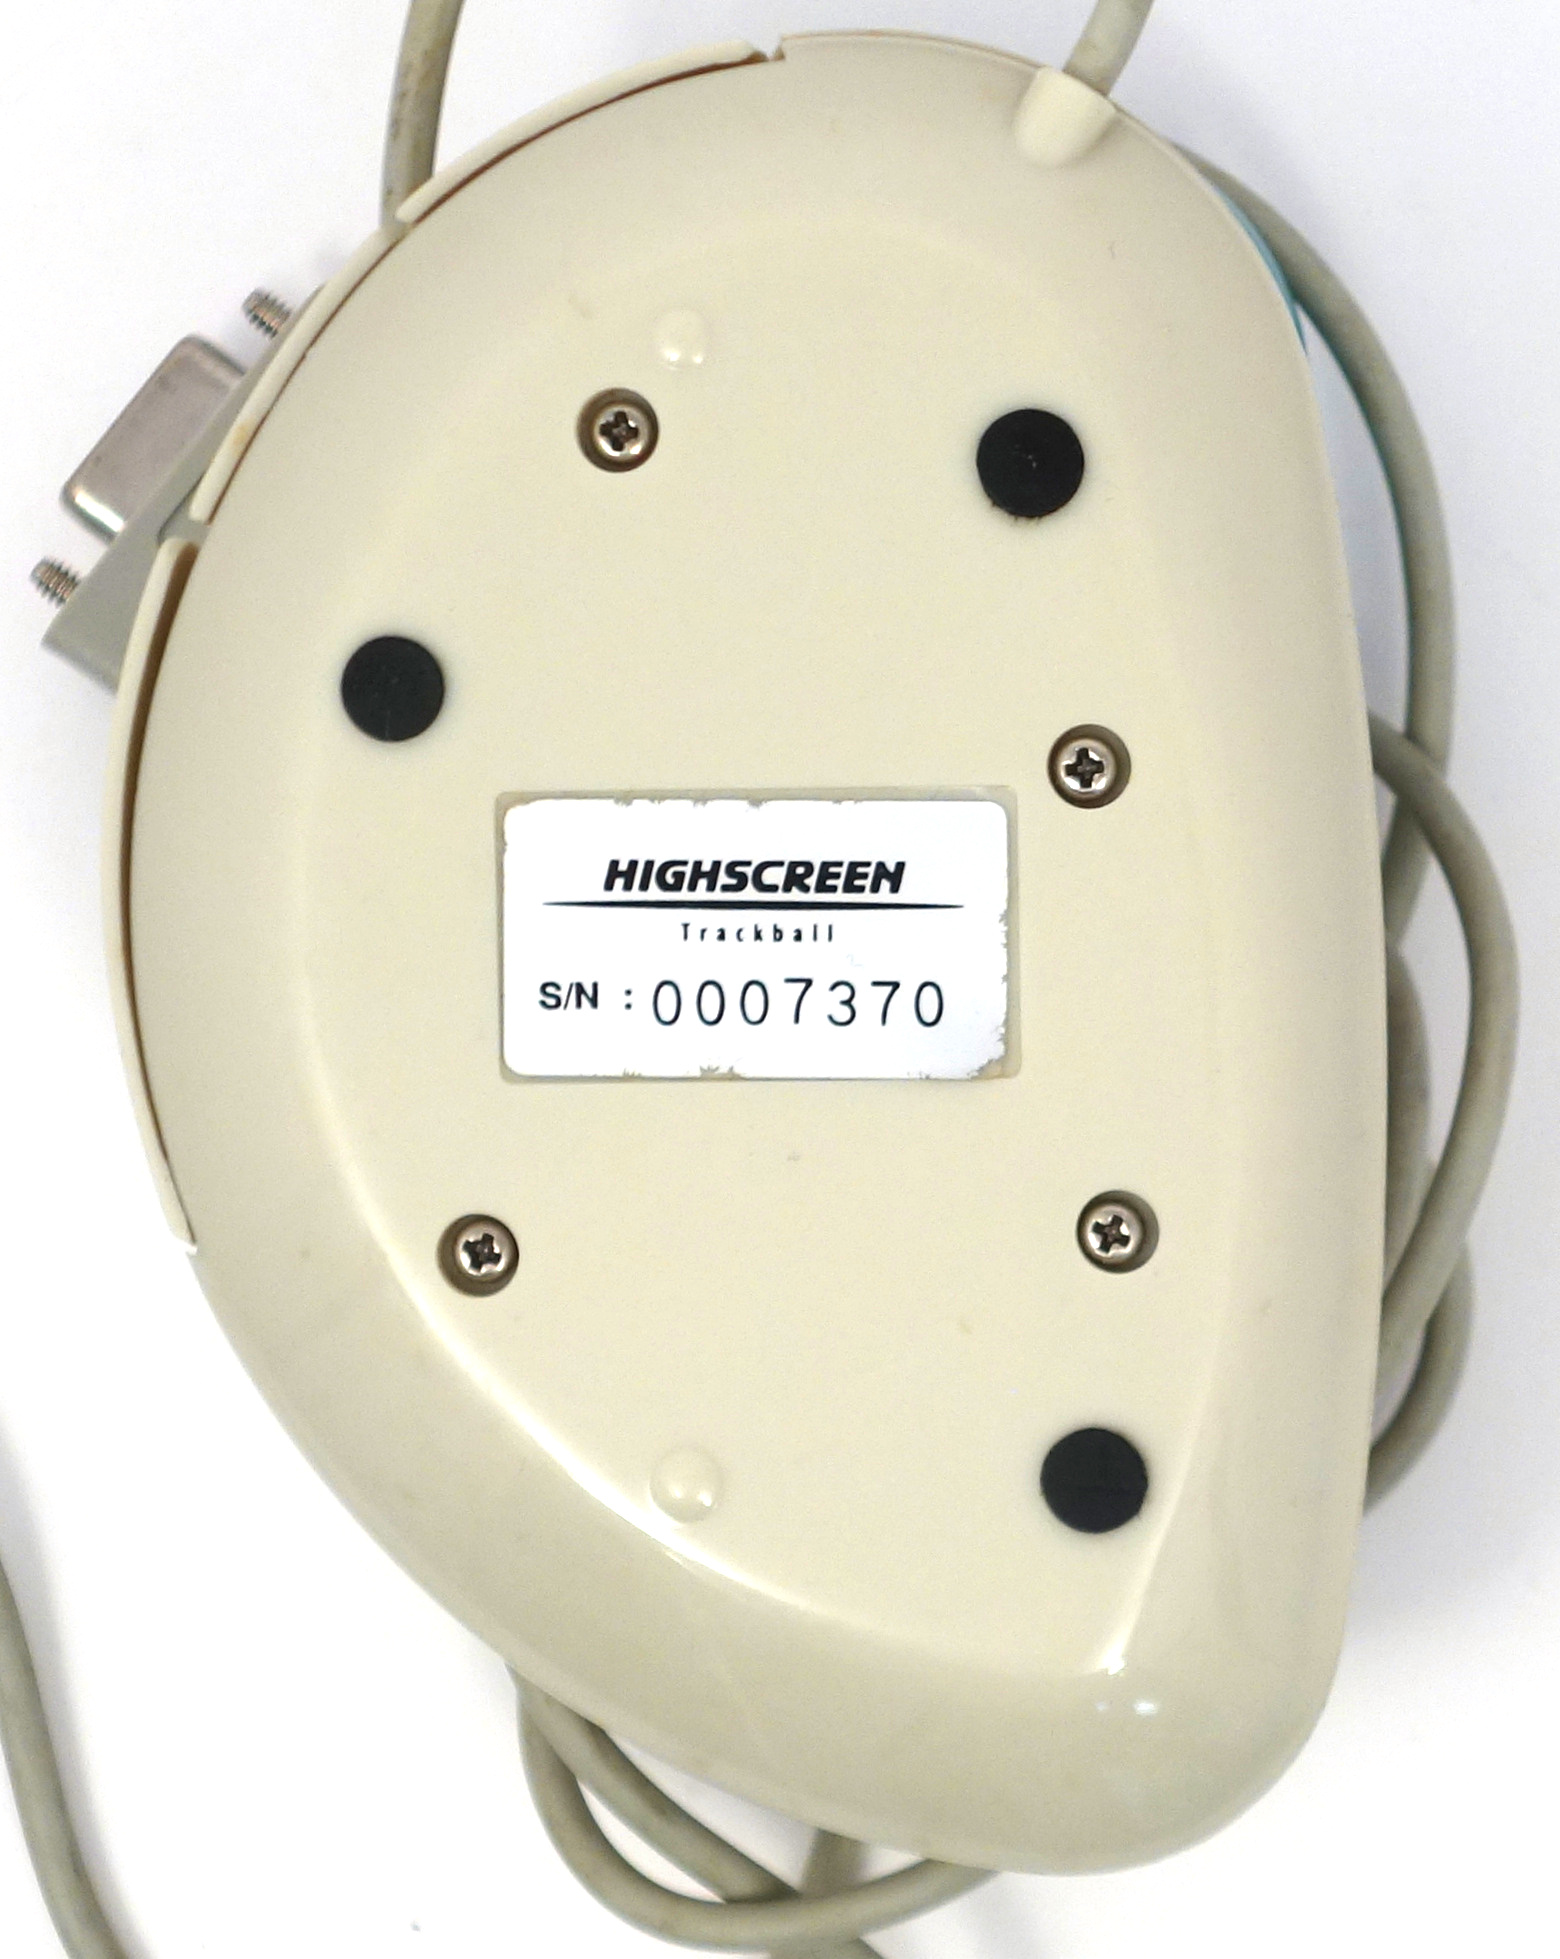
\includegraphics[scale=0.39]{1993_colani_trackball/bottom_w_30.jpg}

    \caption{Colani Trackball, вид сверху и снизу}
    \label{fig:ColaniTopBottom}
\end{figure}

Начиная с концепт-каров, всячески подчеркивавших аэродинамику высоких скоростей, Луиджи Колани развил собственный новый стиль индустриального дизайна "--- бионику. Главный принцип бионики "--- придание предметам округлости и обтекаемых природных форм (рис. \ref{fig:ColaniTopBottom}).

В целом, дизайнер признавал первичность функции предмета перед его формой. Однако раз за разом он не мог устоять перед возможностью сделать изделие более <<природным>>, снабдить его изгибами, подчас сменяющими друг друга самым неожиданным образом, наводящим на мысли о скалах, подверженных длительной работе ветра или волн. В консервативных отраслях, например в автомобилестроении, такой подход обоснованно воспринимался как чересчур эксцентричный. Однако применительно к средствам управления курсором он оказался предвестником новой эры эргономичных мышей со сложной асимметричной формой, рассчитанной на максимально комфортное положение руки человека. Этой тенденции способствовало как то, что подобные формы легко воспроизводятся при литье пластиковых корпусов манипуляторов (чего нельзя сказать, например, о кузовах автомобилей), так и популярность глиняных моделей со следами сжимавшей их руки, позволявших разработчику без больших сложностей получить анотомически-точное и необычное внешне изделие.

Однако по всей видимости сам Луиджи Колани не прибегал к такому способу получения формы. Как можно видеть на рис. \ref{fig:ColaniSize} и \ref{fig:ColaniHand}, Colani Trackball является весьма компактным изделием, почти целиком помещающимся в ладони.

\begin{figure}[h]
    \centering
    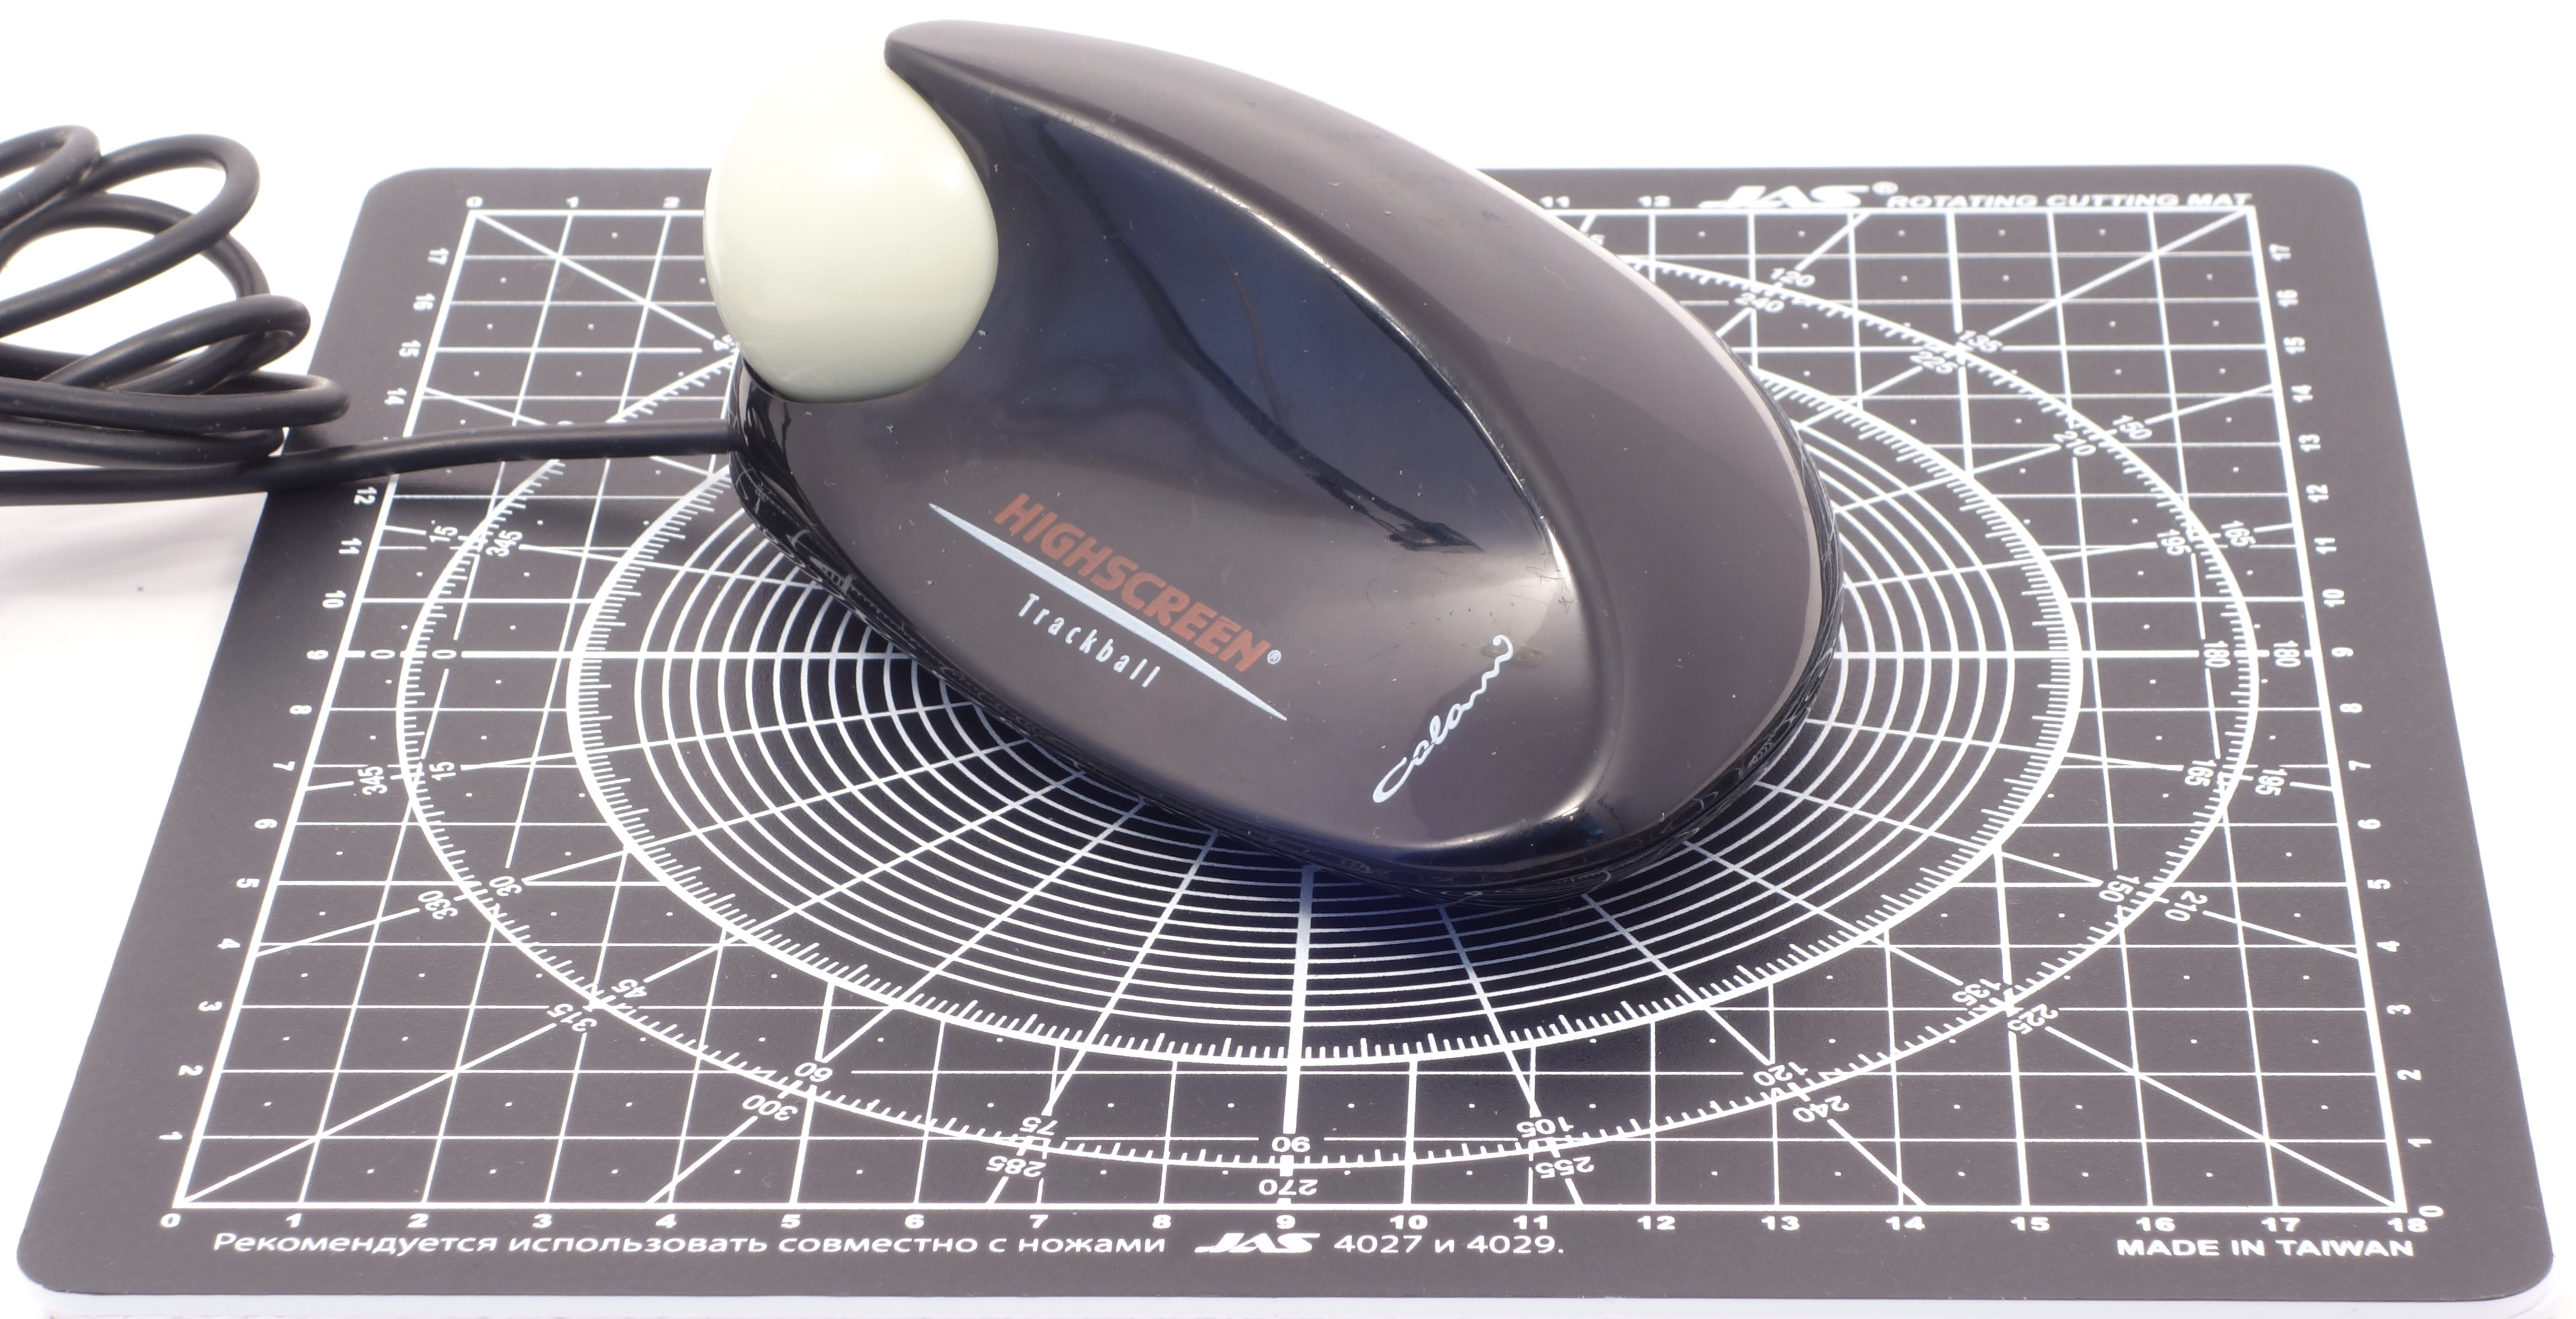
\includegraphics[scale=0.5]{1993_colani_trackball/size_30.jpg}
    \caption{Colani Trackball на размерном коврике с шагом сетки 1 см}
    \label{fig:ColaniSize}
\end{figure}

Вогнутая часть корпуса практически не работает в качестве опоры для кисти, а в основном несет эстетическую и художественную функцию (что, впрочем, можно сказать об абсолютном большинстве дизайнерских манипуляторов). Вместе с тем, положение руки на трекболе является удобным, клавиши расположены в хорошей доступности и имеют достаточную площадь, а шар сильно выдается из корпуса, что делает его вращение более удобным (конечно, если пользователь до него дотянется).

\begin{figure}[h]
    \centering
    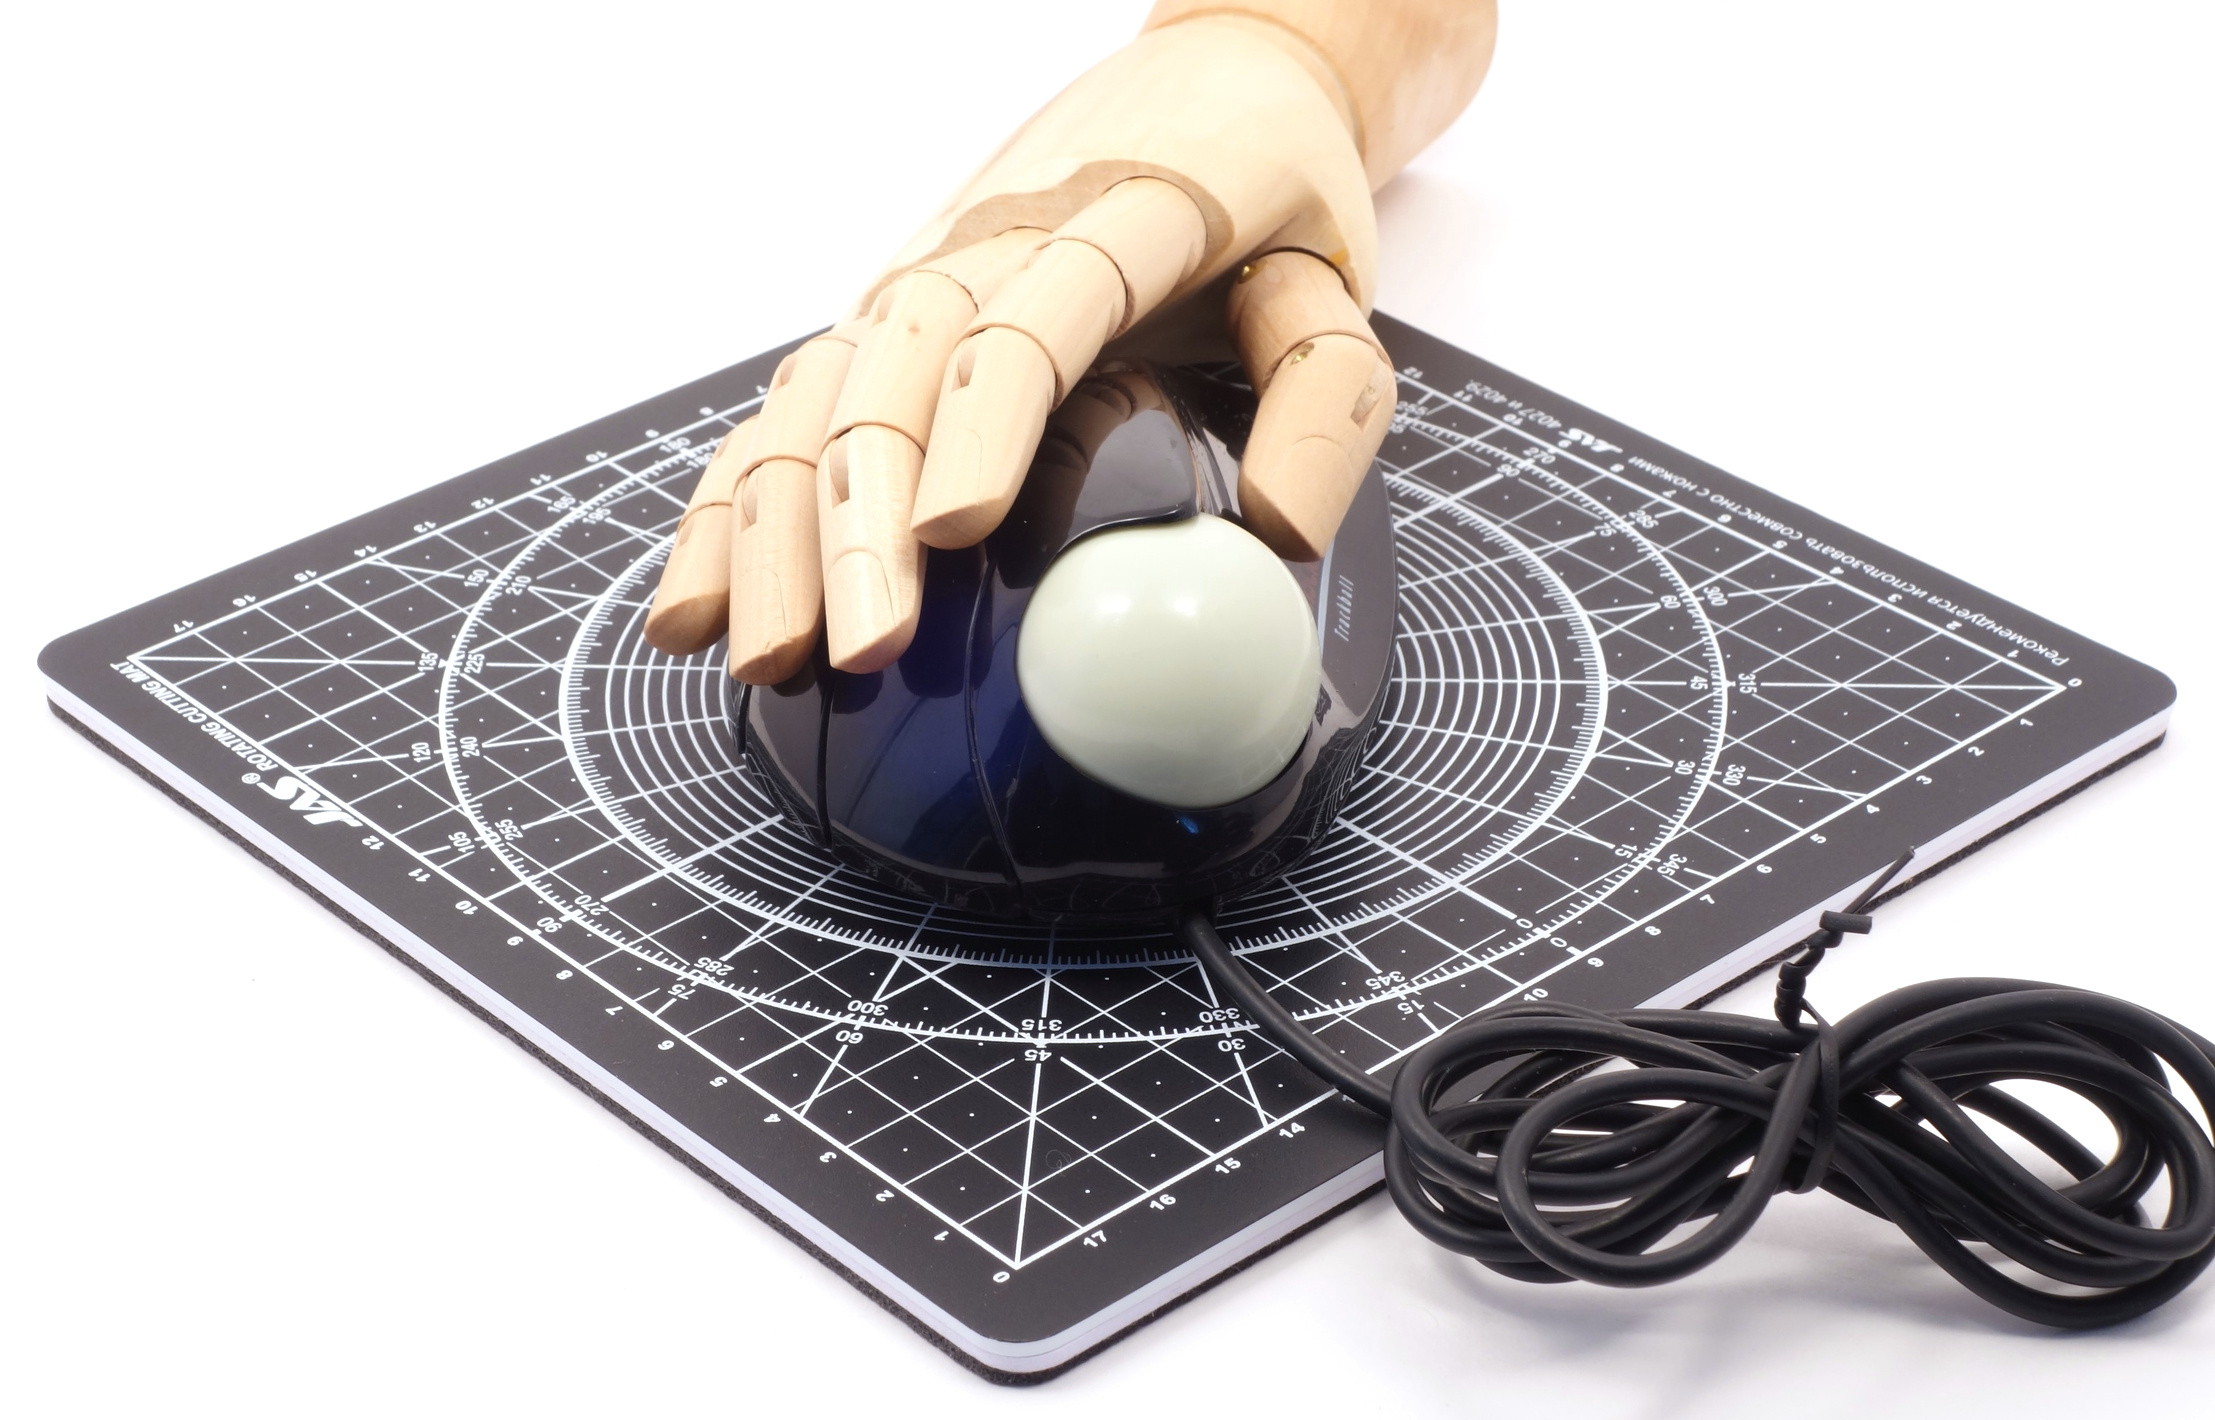
\includegraphics[scale=0.15]{1993_colani_trackball/hand_60.jpg}
    \caption{Colani Trackball в комплекте с моделью руки человека}
    \label{fig:ColaniHand}
\end{figure}

Внутреннее устройство трекбола, показанное на рис. \ref{fig:ColaniInside}, позволяет классифицировать его как оптомеханический, с зубчатыми дисками энкодеров, характерными для конца 80-х "--- начала 90-х годов. Заметим, что выбор деталей является чрезвычайно бюджетным: трекбол содержит минимум подвижных частей и минимум металлических деталей (к числу последних можно отнести только оси энкодоров, прижимную пружину и расположенную под печатной платой металлическую пластину-утяжелитель).

\begin{figure}[h]
    \centering
    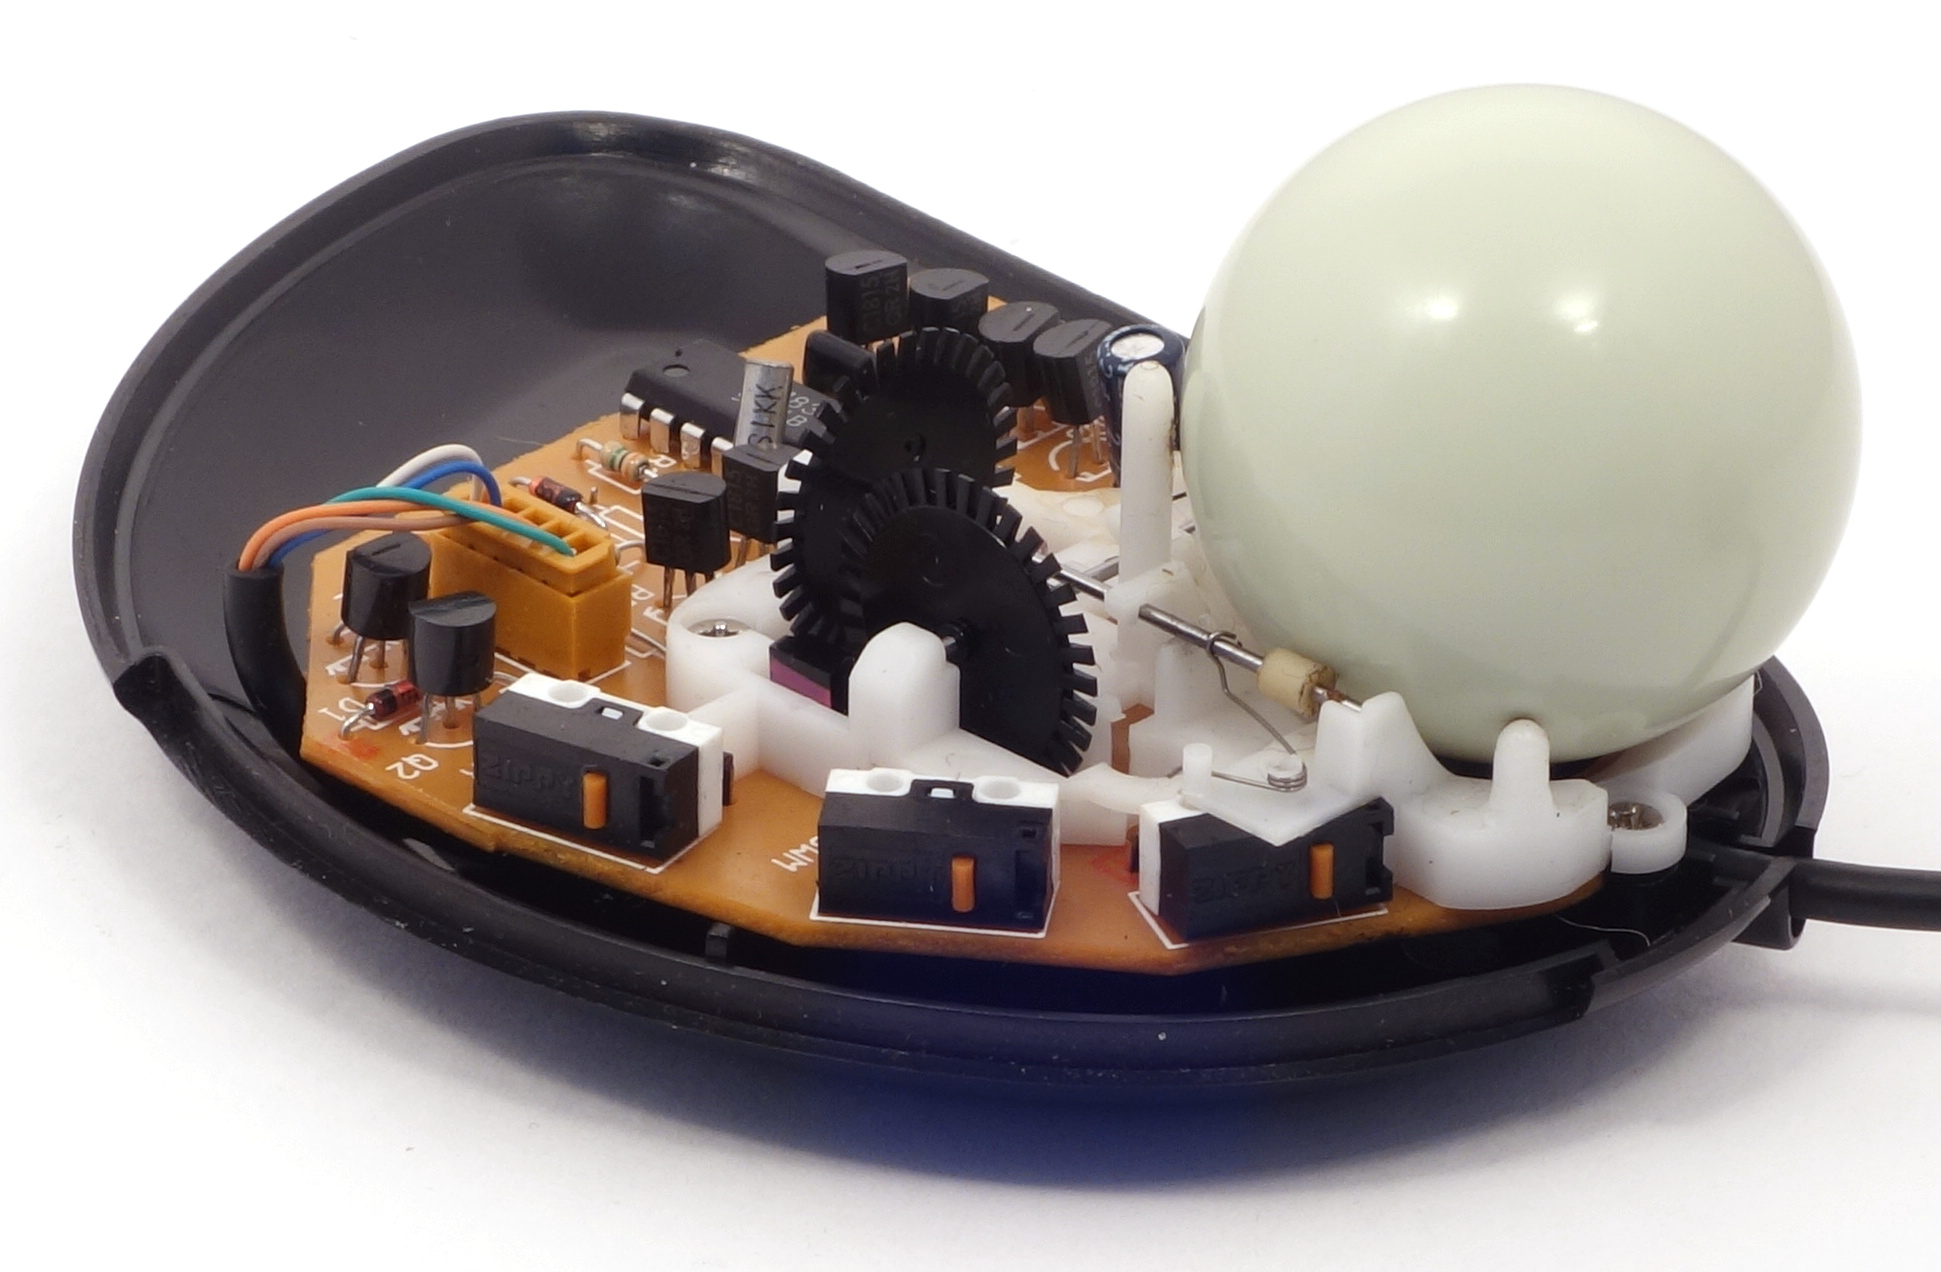
\includegraphics[scale=0.8]{1993_colani_trackball/inside_30.jpg}
    \caption{Colani Trackball в разобранном виде}
    \label{fig:ColaniInside}
\end{figure}

\begin{thebibliography}{9}
    \bibitem {wiki} Luigi Colani – Wikipedia \url{https://en.wikipedia.org/wiki/Luigi_Colani}
    \bibitem {award} iF – HIGHSCREEN Colani Trackball \url{https://ifdesign.com/en/winner-ranking/project/highscreen-colani-trackball/19311}
\end{thebibliography}

\end{document}
